% ****** Start of file apssamp.tex ******
%
%   This file is part of the APS files in the REVTeX 4.1 distribution.
%   Version 4.1r of REVTeX, August 2010
%
%   Copyright (c) 2009, 2010 The American Physical Society.
%
%   See the REVTeX 4 README file for restrictions and more information.
%
% TeX'ing this file requires that you have AMS-LaTeX 2.0 installed
% as well as the rest of the prerequisites for REVTeX 4.1
%
% See the REVTeX 4 README file
% It also requires running BibTeX. The commands are as follows:
%
%  1)  latex apssamp.tex
%  2)  bibtex apssamp
%  3)  latex apssamp.tex
%  4)  latex apssamp.tex
%
\documentclass[%
 reprint,
%superscriptaddress,
%groupedaddress,
%unsortedaddress,
%runinaddress,
%frontmatterverbose,
%preprint,
%showpacs,preprintnumbers,
%nofootinbib,
%nobibnotes,
%bibnotes,
 amsmath,amssymb,
 aps,
pra,
%prb,
%rmp,
%prstab,
%prstper,
%floatfix,
]{revtex4-1}

\usepackage{graphicx}% Include figure files
\usepackage{dcolumn}% Align table columns on decimal point
\usepackage{bm}% bold math
\usepackage{enumitem}
% Stuff for Mogens' nice figure
\usepackage{braket}
\usepackage{tikz}


% Stuff for showing the algorithms
\usepackage{algorithm}
\usepackage[noend]{algpseudocode}

\newcommand{\dif}[2]{\frac{\text{d} #1}{\text{d} #2}}
\newcommand{\diff}[2]{\frac{\partial #1}{\partial #2}}
\DeclareMathOperator*{\argmin}{arg\,min}

\newcommand{\procspie}{Proceedings of the SPIE}
%\usepackage{hyperref}% add hypertext capabilities
%\usepackage[mathlines]{lineno}% Enable numbering of text and display math
%\linenumbers\relax % Commence numbering lines

%\usepackage[showframe,%Uncomment any one of the following lines to test
%%scale=0.7, marginratio={1:1, 2:3}, ignoreall,% default settings
%%text={7in,10in},centering,
%%margin=1.5in,
%%total={6.5in,8.75in}, top=1.2in, left=0.9in, includefoot,
%%height=10in,a5paper,hmargin={3cm,0.8in},
%]{geometry}

\begin{document}

%\preprint{APS/123-QED}

\title{Gradient-Based Optimal Control of Quantum Many-body Systems in Optical Lattices}% Force line breaks with \\

\author{J. J. W. H. S\o rensen}
\author{F. S. M\o ller}
\author{J. F. Sherson}
\affiliation{Aarhus University}
\email{sherson@phys.au.dk}
\date{\today}% It is always \today, today,
             %  but any date may be explicitly specified

\begin{abstract}
Abstract ...


\end{abstract}

\maketitle

\section{Introduction}

\section{Control Derivatives}



\section{Results}


\begin{figure}[h!]
    \centering
    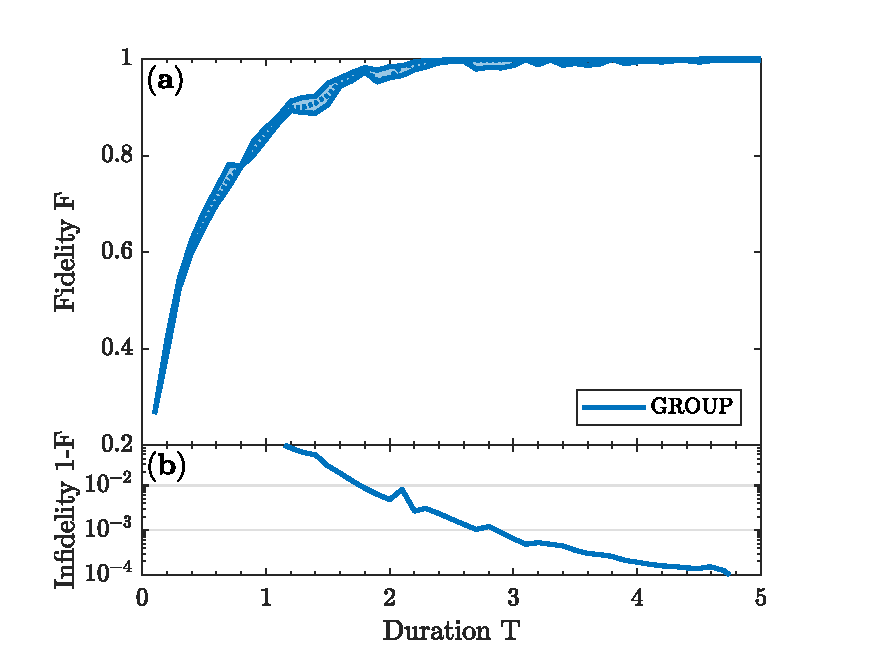
\includegraphics[width=0.8\textwidth]{Figures/FidelityDuration.pdf}
    \caption{\textit{Final fidelity obtained for optimal control at various durations. \textbf{(a)} the dotted line marks the median fidelity achieved, while the shaded area displays the $25\%$- and $75\%$-quartiles of the solutions. \textbf{(b)} the lowest infidelity achieved for each duration. }}
    \label{fig:FidelityDuration}
\end{figure}

\begin{figure}[h!]
    \centering
    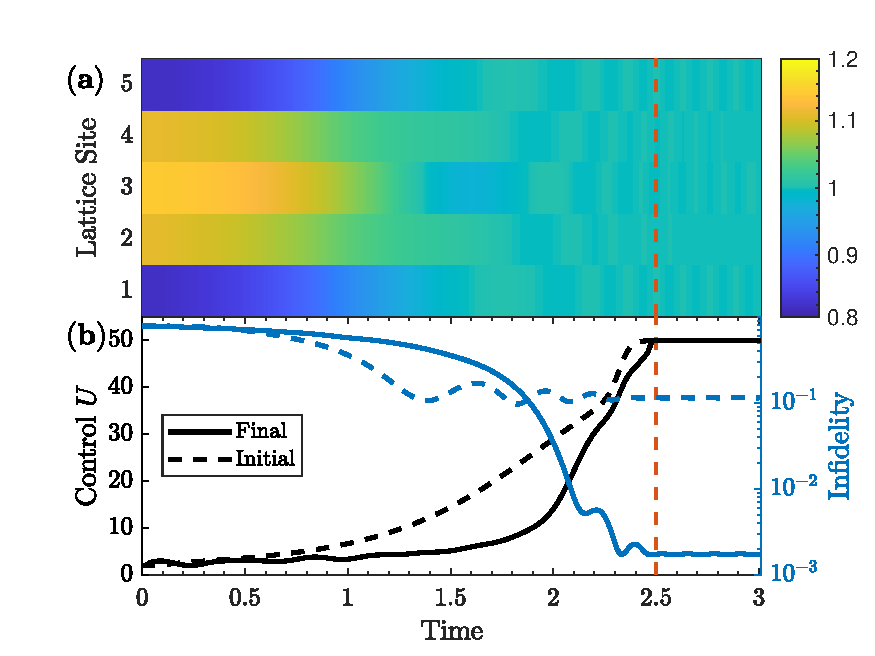
\includegraphics[width=0.8\textwidth]{Figures/OptRamp.pdf}
    \caption{\textit{Solution with highest fidelity achieved for duration $T = 2.5$. The dashed, red line marks the end of the duration, from which the system is further evolved using the final control value. \textbf{(a)} logarithmically scaled expectation value of the number operator, $\braket{\hat{n}_i}$, for each site, as the system is evolved according to the optimized ramp. \textbf{(b)} the initial and optimized ramp sequences along with the corresponding evolution of fidelities.}}
    \label{fig:OptRamp}
\end{figure}

\begin{figure}[h!]
    \centering
    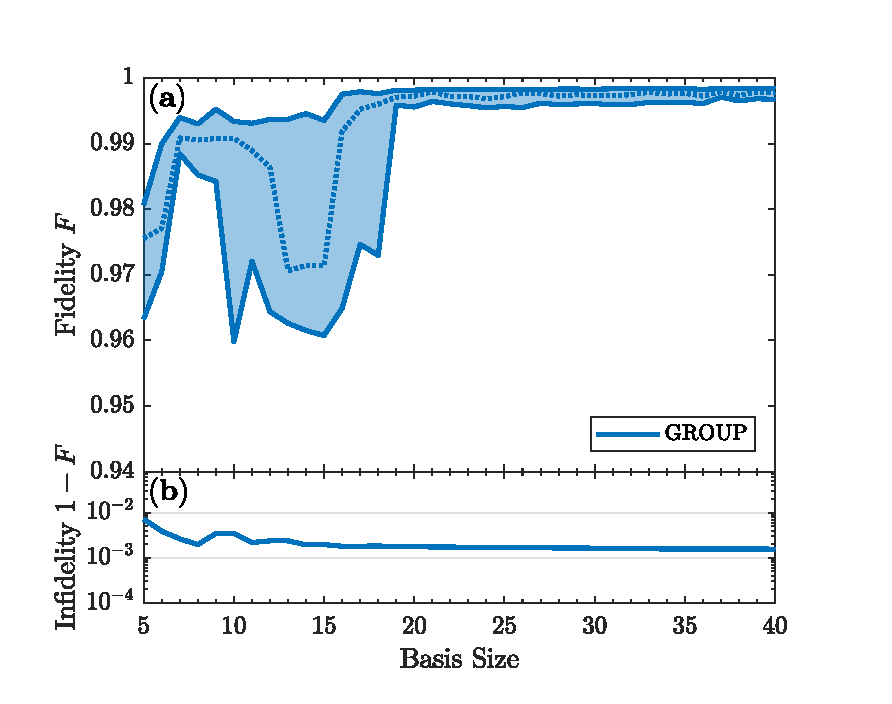
\includegraphics[width=0.8\textwidth]{Figures/FidelityBasisSize.pdf}
    \caption{\textit{Final fidelity obtained for optimal control at various optimization space dimensions for duration $T = 2.5$. \textbf{(a)} the dotted line marks the median fidelity achieved, while the shaded area displays the $25\%$- and $75\%$-quartiles of the solutions. \textbf{(b)} the lowest infidelities achieved for each basis size.}}
    \label{fig:FidelityBasisSize}
\end{figure}

\begin{figure}[h!]
    \centering
    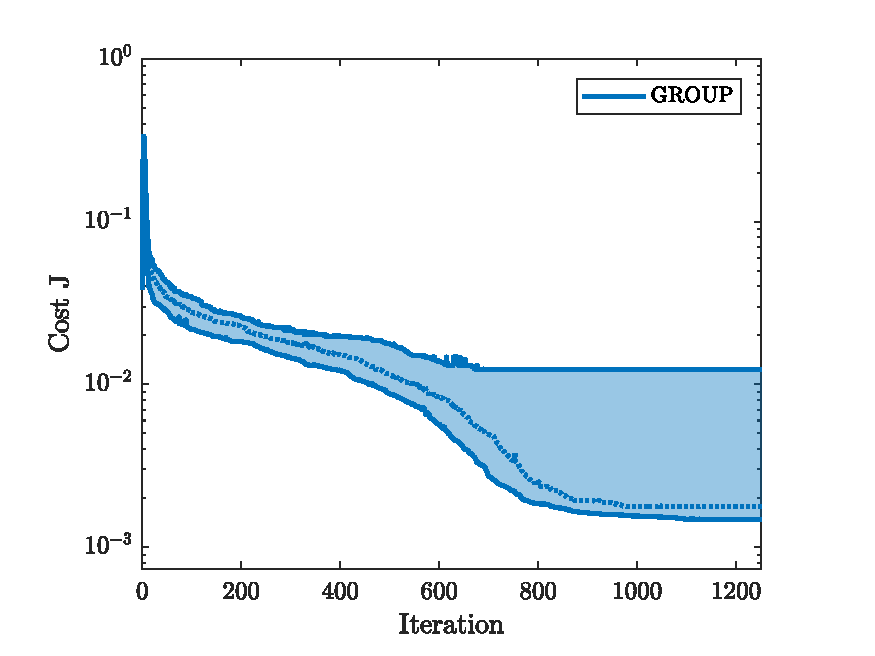
\includegraphics[width=0.8\textwidth]{Figures/CostProgress.pdf}
    \caption{\textit{The value of the cost function at a given number of time evolutions. The dotted line marks the median and the shaded area indicates the $25\%$- and $75\%$-quartiles found from X different random initial controls.}}
    \label{fig:FidelityBasisSize5}
\end{figure}


%\bibliographystyle{apsrev4-1}
%\bibliography{references}

\end{document}
%
% ****** End of file apssamp.tex ******
